% Created 2024-04-21 Sun 21:36
% Intended LaTeX compiler: pdflatex
\documentclass[bigger]{beamer}
\usepackage[utf8]{inputenc}
\usepackage[T1]{fontenc}
\usepackage{graphicx}
\usepackage{longtable}
\usepackage{wrapfig}
\usepackage{rotating}
\usepackage[normalem]{ulem}
\usepackage{amsmath}
\usepackage{amssymb}
\usepackage{capt-of}
\usepackage{hyperref}
\usetheme{default}
\author{Alexander Brown}
\date{\today}
\title{A SIMULATED ANNEALING APPROACH TO THE BATTERY ELECTRIC BUS CHARGING PROBLEM}
\AtBeginSection{\frame{\sectionpage}}
\hypersetup{
 pdfauthor={Alexander Brown},
 pdftitle={A SIMULATED ANNEALING APPROACH TO THE BATTERY ELECTRIC BUS CHARGING PROBLEM},
 pdfkeywords={},
 pdfsubject={},
 pdfcreator={Emacs 29.3 (Org mode 9.6.15)}, 
 pdflang={English}}
\begin{document}

\maketitle
\begin{frame}{Outline}
\tableofcontents
\end{frame}


\section{Introduction}
\label{sec:org312b084}
\begin{frame}[label={sec:orgf160924}]{Problem Description}
\begin{columns}
\begin{column}{0.5\columnwidth}
\begin{itemize}
\item total of \(n_A\) buses in the fleet
\item \(n_V\) visits\footnote{A visit describes when a bus arrives, assigned a charge queue, and then departs} to the station divided between the \(n_A\) buses
\item Each bus in initialized with a charge of \(\alpha_b \kappa_i\)
\end{itemize}
\end{column}

\begin{column}{0.5\columnwidth}
\begin{itemize}
\item After each visit the bus goes on its route and discharges by \(\Delta_i\)
\item The charge is not allowed to go below \(\nu_b \kappa_i\) during operational hours
\item Each bus is required to finish the day with a minimum charge of \(\beta_b \kappa_i\)\footnote{PAP application only}
\end{itemize}
\end{column}
\end{columns}
\end{frame}

\begin{frame}[label={sec:orgfd5618f}]{Mixed Integer Linear Programming}
\begin{align*}
\text{max }        &J = \sum_j c_j x_j + \sum_k d_k y_k&         &               \\
\text{subject to } &\sum_j a_{ij} x_j + \sum_k g_{ik} y_k \le b_i&  &(i = 1,2,...,m)\\
                  &x_j \ge 0&                              &(j = 1,2,...,n)\\
                  &y_k \in \mathbb{Z^+}&                   &(k = 1,2,...,n)\\
\end{align*}

\begin{itemize}
\item \(J\): Objective function
\item \(x_j \in \mathbb{R}\) and \(y_k \in \mathbb{Z}^+\): Decision Variables
\item \(c_j, d_k, a_{ij}, g_{ik}, b_i \in \mathbb{R}\): Parameters
\end{itemize}
\end{frame}

\begin{frame}[label={sec:org61ecc3f}]{The Berth Allocation Problem\footnote{\url{https://www.mdpi.com/2077-1312/11/7/1280}}}
\begin{figure}[htpb]
\centering
    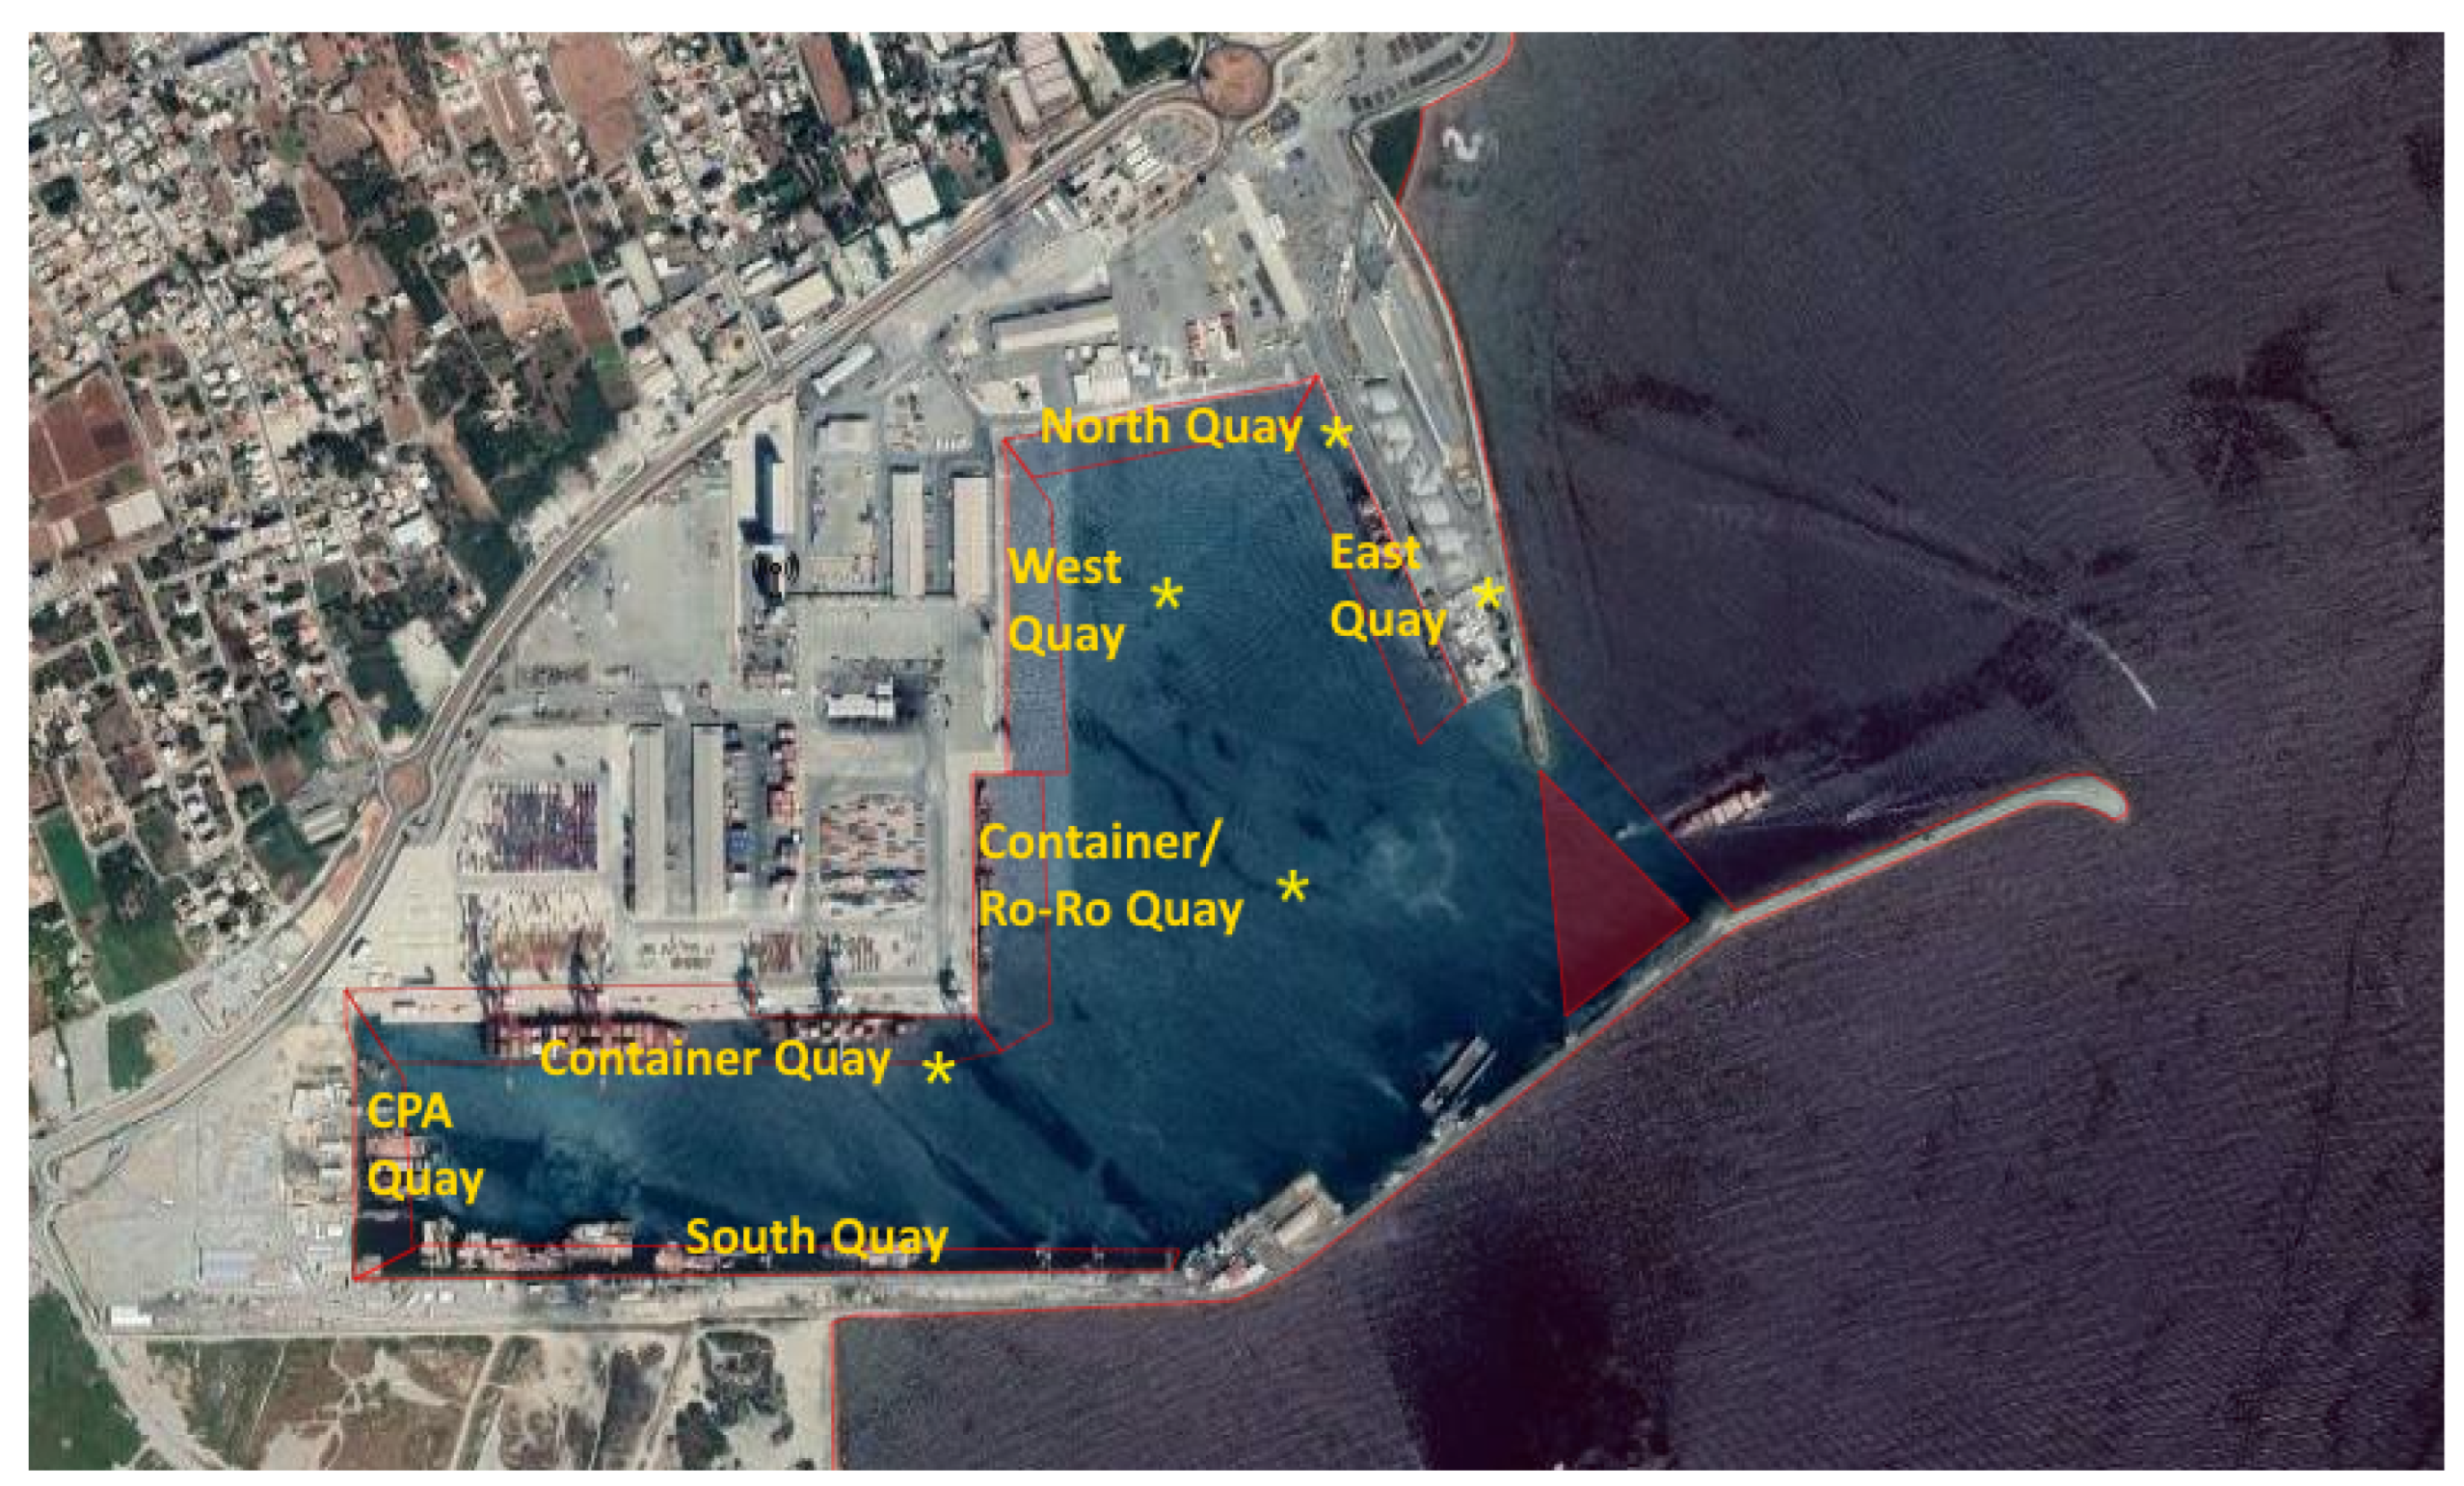
\includegraphics[width=0.9\textwidth]{img/berthing-sky-picture}
\end{figure}
\end{frame}

\begin{frame}[label={sec:org98dcbdc}]{The Berth Allocation Problem}
\begin{columns}
\begin{column}{0.5\columnwidth}
\begin{itemize}
\item Vessels move down toward the quay
\item Recieve service
\item Exit to the right
\end{itemize}
\end{column}

\begin{column}{0.5\columnwidth}
\begin{figure}[htpb]
\centering
    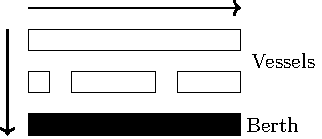
\includegraphics{img/bap}
    \label{subfig:bapexample}
\end{figure}
\end{column}
\end{columns}
\end{frame}

\begin{frame}[label={sec:org149e1b1}]{The Berth Allocation Problem}
\begin{itemize}
\item A variant of the rectangle packing problem
\item Solves the problem of optimally assigning incoming vessels to be serviced
\begin{itemize}
\item \(\mathbb{O}\): Spatiotemporal allocations for vessels
\item \(O\): Time horizon and berthing space
\end{itemize}
\end{itemize}


\begin{figure}[htpb]
\centering
    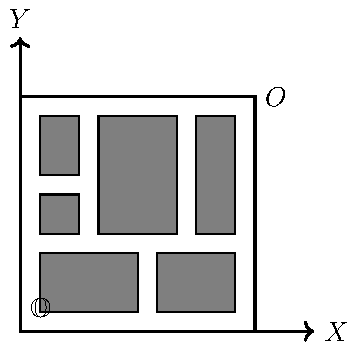
\includegraphics[width=0.5\textwidth]{img/spatiotemporal-packing}
\end{figure}
\end{frame}

\begin{frame}[label={sec:orgfb7912f}]{The Position Allocation Problem}
\begin{columns}
\begin{column}{0.5\columnwidth}
\begin{itemize}
\item Service flow is left to right
\item Single charger type
\item All arrivals are considered unique
\item Service times are assumed to be known
\end{itemize}
\end{column}

\begin{column}{0.5\columnwidth}
\begin{figure}[htpb]
\centering
    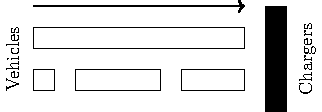
\includegraphics{img/pap}
    \label{subfig:papexample}
\end{figure}
\end{column}
\end{columns}
\end{frame}

\section{The Position Allocation Problem Approach With Linear Battery Dynamic}
\label{sec:orge593a11}
\begin{frame}[label={sec:orgac98189}]{Requirements for BEB implementation}
\begin{itemize}
\item Charges must be able to be tracked
\item Service time is unknown
\item Accommodate chargers of different speeds
\item Minimize charger count
\item Minimize consumption cost
\item Encourage slow charger use for battery health
\end{itemize}
\end{frame}

\begin{frame}[label={sec:orga0619d4}]{Objective Function}
\begin{equation*}
\label{eq:objective}
	\min \sum_{i=1}^N \sum_{q=1}^{n_Q} \Big( w_{iq} m_q + g_{iq} \epsilon_q \Big)
\end{equation*}

\begin{itemize}
\item \(w_{iq} m_q\): Assignment cost
\item \(g_{iq} \epsilon_q\): Consumption cost
\end{itemize}
\end{frame}

\begin{frame}[label={sec:org953b413}]{Packing Constraints}
\begin{columns}
\begin{column}{0.5\columnwidth}
\begin{itemize}
\item Used to ensure that individual rectangles do not overlap
\item \(\sigma_{ij}\) establishes temporal ordering when active
\item \(\psi_{ij}\) establishes spacial ordering when active
\end{itemize}
\end{column}

\begin{column}{0.5\columnwidth}
\begin{equation*}
    u_j - u_i - s_i - (\sigma_{ij} - 1)T \geq 0
\end{equation*}
\begin{equation*}
    v_j - v_i - (\psi_{ij} - 1)n_Q \geq 1
\end{equation*}
\begin{equation*}
    \sigma_{ij} + \sigma_{ji} \leq 1
\end{equation*}
\begin{equation*}
    \psi_{ij} + \psi_{ji} \leq 1
\end{equation*}
\begin{equation*}
    \sigma_{ij} + \sigma_{ji} + \psi_{ij} + \psi_{ji} \geq 1
\end{equation*}
\end{column}
\end{columns}
\end{frame}

\begin{frame}[label={sec:org52cf2b0}]{Packing Constraints}
\begin{columns}
\begin{column}{0.5\columnwidth}
\begin{itemize}
\item Calculates the charge duration
\item Ensures the arrival time is before the initial charge time
\item The initial charge time must be early enough as to not go over the time horizon
\item The detach time must be before the departure time
\end{itemize}
\end{column}

\begin{column}{0.5\columnwidth}
\begin{equation*}
    s_i + u_i = d_i
\end{equation*}
\begin{equation*}
    a_i \leq u_i \leq (T - s_i)
\end{equation*}
\begin{equation*}
    d_i \leq \tau_i
\end{equation*}
\end{column}
\end{columns}
\end{frame}

\begin{frame}[label={sec:orge7d6b60}]{Linear Battery Dynamic Constraints}
\begin{columns}
\begin{column}{0.5\columnwidth}
\begin{itemize}
\item Calculates the charge for the next visit
\item Ensures the current charge is above the minimum charge threshold
\item Ensures the current charge is below the battery capacity
\end{itemize}
\end{column}

\begin{column}{0.5\columnwidth}
\begin{equation*}
    \eta_i + \sum_{q=1}^{n_Q} g_{iq} r_q - \Delta_i = \eta_{\gamma_i}
\end{equation*}
\begin{equation*}
    \eta_i + \sum_{q=1}^{n_Q} g_{iq} r_q - \Delta_i \geq \nu_{\Gamma_i} \kappa_{\Gamma_i}
\end{equation*}
\begin{equation*}
    \eta_i + \sum_{q=1}^{n_Q} g_{iq} r_q \leq \kappa_{\Gamma_i}
\end{equation*}
\end{column}
\end{columns}
\end{frame}

\begin{frame}[label={sec:org8f89b69}]{Bilinear Linearization Constraints}
\begin{columns}
\begin{column}{0.5\columnwidth}
\begin{itemize}
\item Linearization of bilinear terms
\end{itemize}

\begin{equation*}
    \label{eq:giq_cases}
    g_{iq} =
    \begin{cases}
        s_i & w_{iq} = 1 \\
        0 & w_{iq} = 0
    \end{cases}.
\end{equation*}
\end{column}


\begin{column}{0.5\columnwidth}
\begin{equation*}
    s_i - (1 - w_{iq})M \leq g_{iq}
\end{equation*}
\begin{equation*}
    s_i \geq g_{iq}
\end{equation*}
\begin{equation*}
    Mw_{iq} \geq g_{iq}
\end{equation*}
\begin{equation*}
    0 \leq g_{iq}
\end{equation*}
\end{column}
\end{columns}
\end{frame}

\begin{frame}[label={sec:orgc3af91c}]{Charging Queue Constraints}
\begin{columns}
\begin{column}{0.5\columnwidth}
\begin{itemize}
\item Ensure only one queue is selected per visit
\item Convert vector representation of queue selection to an integer
\end{itemize}
\end{column}

\begin{column}{0.5\columnwidth}
\begin{equation*}
    \sum_{q=1}^{n_Q} w_{iq} = 1
\end{equation*}
\begin{equation*}
    v_i = \sum_{q=1}^{n_Q} qw_{iq}
\end{equation*}
\end{column}
\end{columns}
\end{frame}


\begin{frame}[label={sec:org48074fa}]{Results}
\begin{itemize}
\item Executed for 7200 seconds (2 hours)
\item \(T = 24\)
\item \(n_V = 338\)
\item \(n_A = 35\)
\item \(\alpha_i = 90\%\);  \(\nu_i = 20\%\);  \(\beta_i = 70\%\)
\item \(\forall q \in \{n_B + 1, n_B + 2,..., n_B + n_C \}; m_q = 1000q\)
\end{itemize}
\end{frame}

\begin{frame}[label={sec:orge28bda6}]{Results}
\begin{figure}[htpb]
\centering
    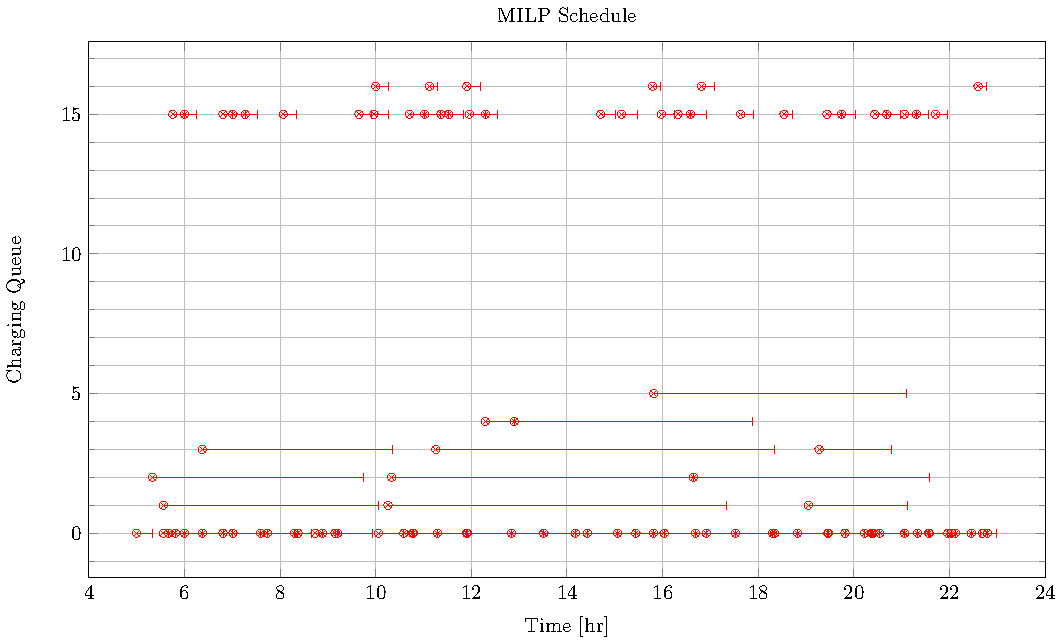
\includegraphics[width=0.6\textwidth]{img/schedule-milp-pap}
\end{figure}
\begin{figure}[htpb]
\centering
    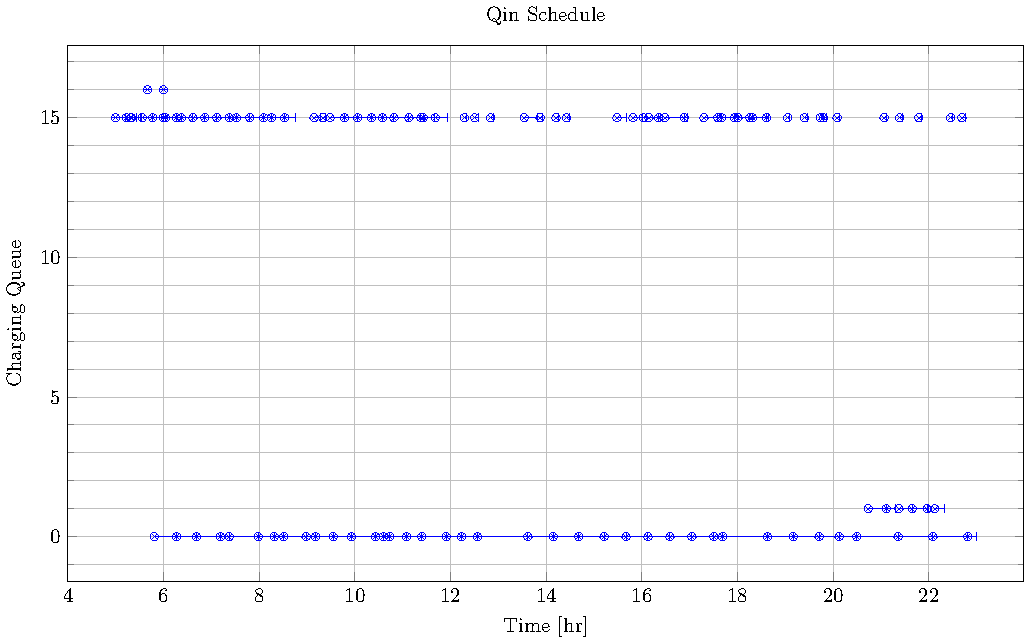
\includegraphics[width=0.6\textwidth]{img/schedule-qin}
\end{figure}
\end{frame}

\begin{frame}[label={sec:org538fd7f}]{Results}
\begin{figure}[htpb]
\centering
    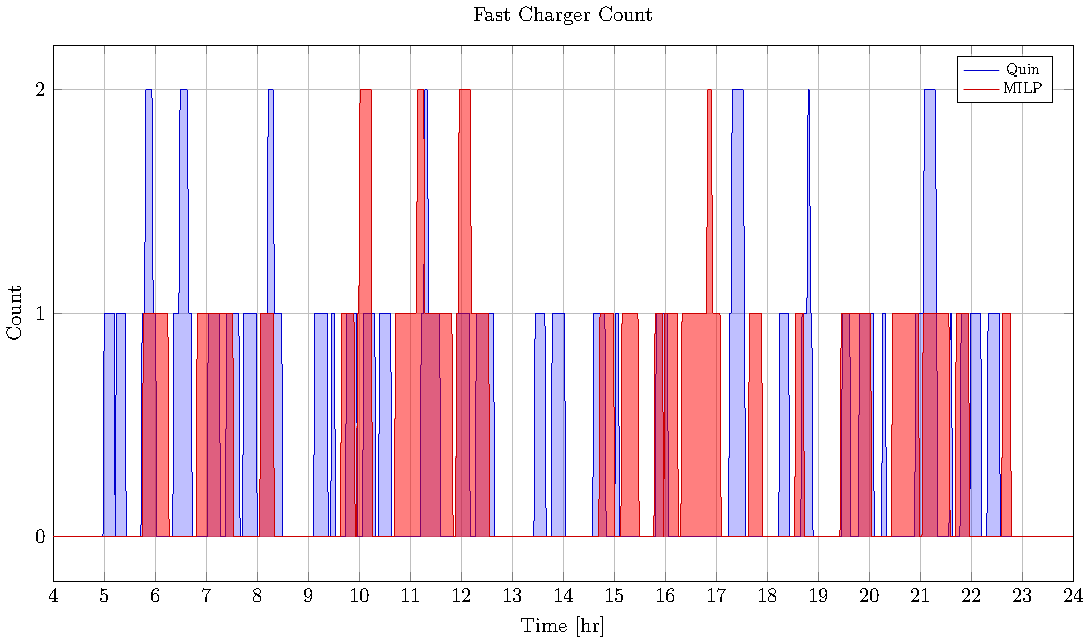
\includegraphics[width=0.6\textwidth]{img/charger-count-fast-milp-pap}
\end{figure}
\begin{figure}[htpb]
\centering
    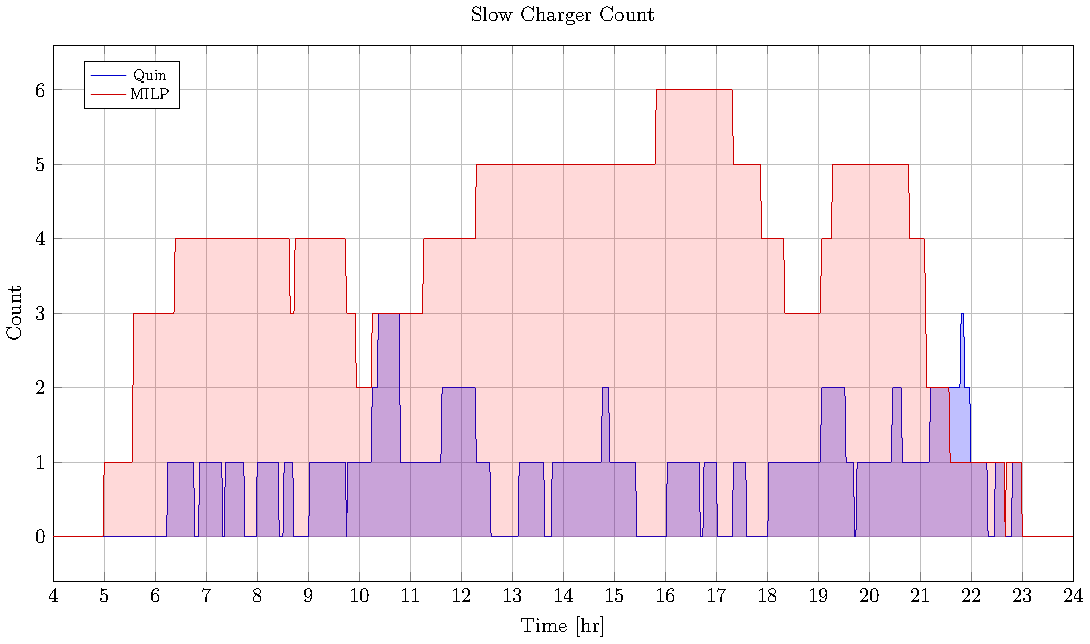
\includegraphics[width=0.6\textwidth]{img/charger-count-slow-milp-pap}
\end{figure}
\end{frame}

\begin{frame}[label={sec:org997a1a5}]{Results}
\begin{figure}[htpb]
\centering
    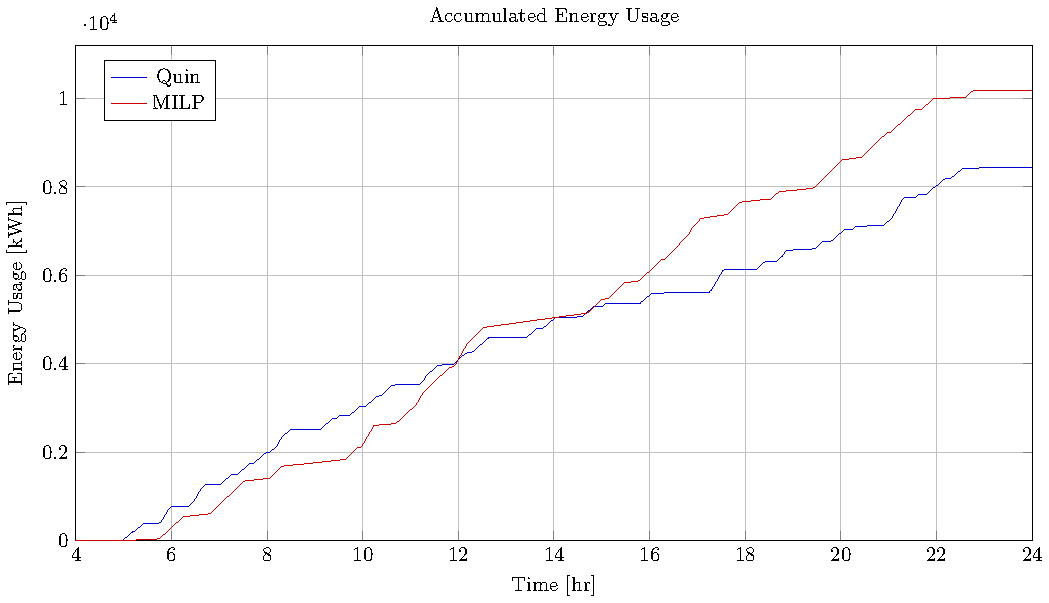
\includegraphics[width=0.6\textwidth]{img/energy-milp-pap}
\end{figure}
\begin{figure}[htpb]
\centering
    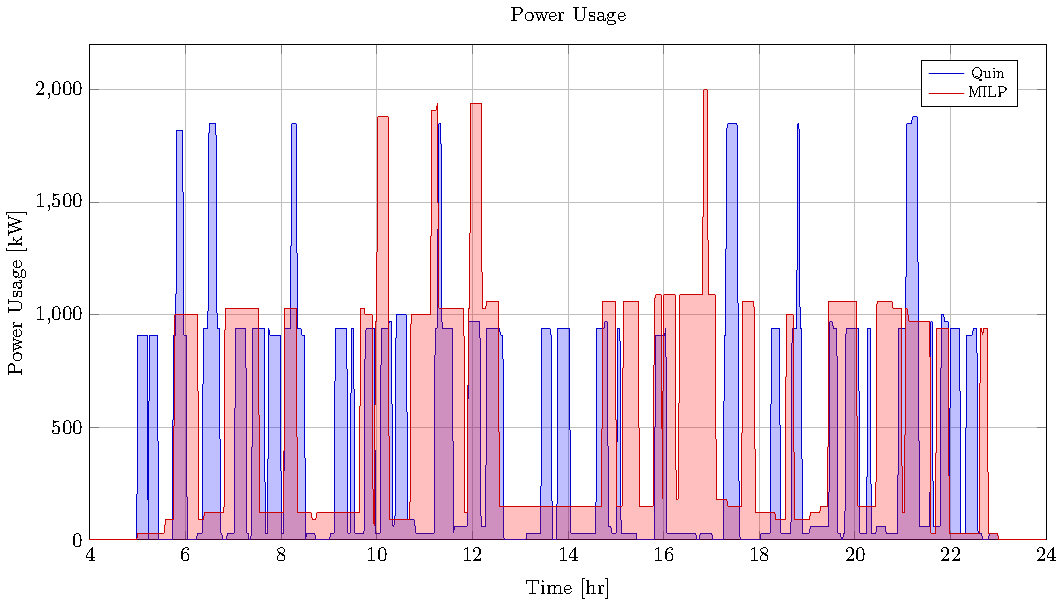
\includegraphics[width=0.6\textwidth]{img/power-milp-pap}
\end{figure}
\end{frame}

\section{The Simulated Annealing Approach With Linear Battery Dynamics}
\label{sec:orgfb47929}
\begin{frame}[label={sec:org14409c9}]{Simulated Annealing}
\begin{itemize}
\item Named after its analogized process where a crystalline solid is heated then allowed to cool at a slow rate until it achieves its most regular possible crystal lattice configuration
\item The algorithm is often applied to problems that contain many local solutions as it employs a stochastic approach that explores the solution space for an approximate global optimum.
\item Within the SA process there are three key components
\begin{itemize}
\item Cooling Schedule
\item Acceptance Criteria
\item Generation Mechanisms
\end{itemize}
\end{itemize}
\end{frame}
\begin{frame}[label={sec:org4acf4ab}]{Cooling Schedule}
\begin{columns}
\begin{column}{0.5\columnwidth}
\begin{itemize}
\item The cooling equation models the rate at which the temperature decreases over time in the SA process.
\item The temperature is high, SA encourages exploration. As the temperature decreases, exploitation is encouraged.
\end{itemize}
\end{column}

\begin{column}{0.5\columnwidth}
\begin{figure}[t!]
  \centering 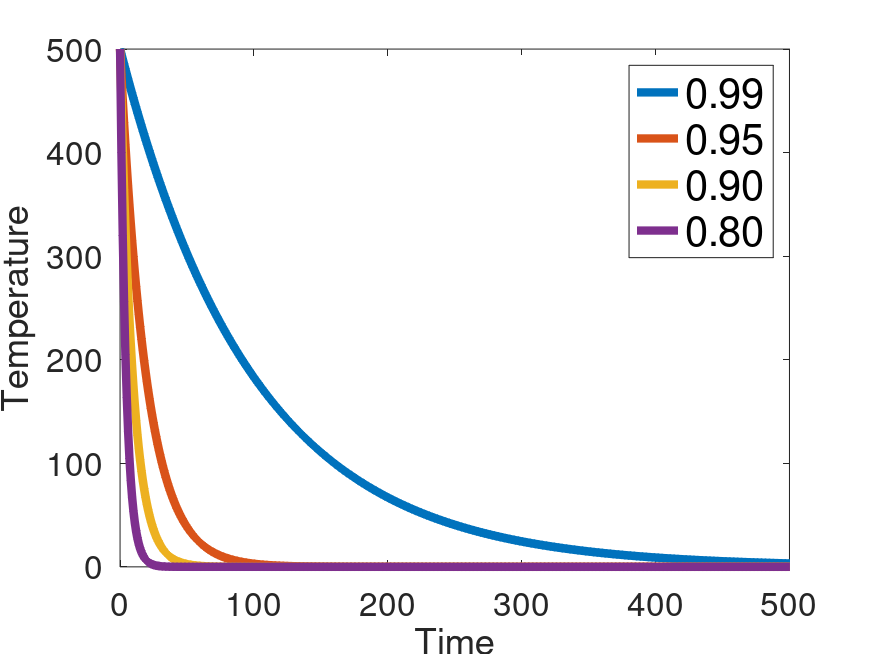
\includegraphics[width=0.9\textwidth]{img/geometric.png}
  \label{fig:geometric}
\end{figure}

\begin{equation*}
t_m = \beta t_{m-1}
\end{equation*}
\end{column}
\end{columns}
\end{frame}

\begin{frame}[label={sec:org8b1b38a}]{Acceptance Criteria}
\begin{equation}
\label{eq:candaccept}
f(\mathbb{I},\bar{\mathbb{I}},t_m) =
\begin{cases}
  1                   & \Delta E > 0 \\
  e^{- \frac{\Delta E}{t_m}} & \text{otherwise}
\end{cases}
\end{equation}
\end{frame}

\begin{frame}[label={sec:org2f39dd3}]{Generation Mechanisms - Primitive Functions}
\begin{itemize}
\item New Visit: Move a bus from a wait queue to charge queue
\item Slide Visit: Change the charge duration of a visit
\item New Charger: Move a visit to a new charger
\item Wait: Move a visit to its idle queue
\item New Window: Execute Wait then New Visit primitives
\end{itemize}
\end{frame}

\begin{frame}[label={sec:org8068f8b}]{Generation Mechanisms - Wrapper Functions}
\begin{itemize}
\item Charge Schedule Generation: Iterate through each visit and execute New Visit
\item Perturb Schedule: Randomly execute one of the primitives with a weighted distribution
\end{itemize}
\end{frame}

\begin{frame}[label={sec:org41f7a0c}]{Objective Function}
\begin{equation*}
  J(\mathbb{I}) = z_d p_d + \sum_{i=1}^{n_V} \Big[ \epsilon_{q_i}r_{q_i} + z_p \phi_i(\eta_i - \nu_{b_i} \kappa_{b_i}) + z_c r_{q_i} s_i \Big]
\end{equation*}

\begin{columns}
\begin{column}{0.5\columnwidth}
\begin{itemize}
\item Demand cost
\begin{itemize}
\item \(p_{T_p}[h] = \frac{1}{T_p} \sum_{h-\frac{T_p}{dt}+1}^h p_h\)
\item \(p_d = \max(p_{fix}, p_{max})\)
\item \(p_{max} = \max\limits_{h \in H}p_{T_p}[h]\)
\end{itemize}
\end{itemize}
\end{column}

\begin{column}{0.5\columnwidth}
\begin{itemize}
\item \(\epsilon_{q_i}r_{q_i}\): Assignment Cost
\item \(z_p \phi_i(\eta_i - \nu_{b_i} \kappa_{b_i})\): Penalty Function
\item \(z_c r_{q_i} s_i\): Consumption Cost
\end{itemize}
\end{column}
\end{columns}
\end{frame}

\begin{frame}[label={sec:org3112b8c}]{Constraints}
\begin{columns}
\begin{column}{0.5\columnwidth}
\begin{equation*}
    \label{seq:c0}
    u_j - d_i - (\sigma_{ij} - 1)T \ge 0
\end{equation*}
\begin{equation*}
    \label{seq:c1}
    q_j - q_i - 1 - (\psi_{ij} - 1)Q \ge 0
\end{equation*}
\begin{equation*}
    \label{seq:c2}
    \sigma_{ij} + \sigma_{ji} \le 1
\end{equation*}
\begin{equation*}
   \label{seq:c3}
    \psi_{ij} + \psi_{ji} \le 1
\end{equation*}
\end{column}

\begin{column}{0.5\columnwidth}
\begin{equation*}
    \label{seq:c4}
    \sigma_{ij} + \sigma_{ji} + \psi_{ij} + \psi_{ji} \ge 1
\end{equation*}
\begin{equation*}
    \label{seq:c5}
    s_i = d_i - u_i
\end{equation*}
\begin{equation*}
    \label{seq:c6}
     \eta_{\xi_i} = \eta_{i} + r_{q_i}s_i - \Delta_i
\end{equation*}
\begin{equation*}
    \label{seq:c7}
    \kappa_{\Xi_i} \geq \eta_{i} + r_{q_i}s_i
\end{equation*}
\begin{equation*}
    \label{seq:c8}
    a_i \leq u_i \leq d_i \le e_i \le \mathcal{T}
\end{equation*}
\end{column}
\end{columns}
\end{frame}

\begin{frame}[label={sec:orgabbde5b}]{Results - What Is In The Thesis}
\begin{itemize}
\item How long it ran for
\item It's sort of working, but not really
\end{itemize}
\end{frame}
\begin{frame}[label={sec:org5b1c91a}]{What Happened?}
\begin{itemize}
\item Score Divergence
\item Difficult Schedules are\ldots{} difficult\ldots{}
\end{itemize}
\end{frame}
\begin{frame}[label={sec:org62c161c}]{How To Resolve This Problem?}
\begin{itemize}
\item Reverse search and weight the visit indices
\end{itemize}
\end{frame}
\begin{frame}[label={sec:org379f22f}]{Results - What Is Not In The Thesis}
\begin{itemize}
\item How long it ra for
\item Plots! WOW!
\end{itemize}
\end{frame}
\section{The Simulated Annealing Approach With Non-Linear Battery Dynamics}
\label{sec:org858de26}
\begin{frame}[label={sec:org0cfc2b0}]{Introduction}
\begin{itemize}
\item Why even consider this?
\item Why use SA
\end{itemize}
\end{frame}
\begin{frame}[label={sec:org1a2136a}]{Non-Linear Battery Dynamics Model}
\begin{itemize}
\item Show function
\item Show plots
\end{itemize}
\end{frame}
\begin{frame}[label={sec:orgc018cc6}]{Results}
\begin{itemize}
\item Figures!
\end{itemize}
\end{frame}
\end{document}
